% \begin{table}[t]
% % \begin{wraptable}{R}{0.5\linewidth}
% \caption{The performance comparison of LLMs for code generation on the MBPP \cite{austin2021program} benchmark, measured by \texttt{Pass@1}. For models with various sizes, we report only the largest size version of each model with the magnitude of \texttt{B} parameters.}
% \label{tab:performance_mbpp}
% \centering
% \scalebox{0.75}{
% \rotatebox{0}{
%     \begin{tabular}{lrc}
%     \toprule
%     \textbf{Model} & \textbf{Size} & \texttt{pass@1} \\ 
% \midrule
%     % GPT-4  & - &    \\ 
%     GPT-3.5-Turbo \cite{gpt-3.5-turbo} & - & 52.2   \\
%     Claude-3-Opus \cite{claude3} & - & 86.4 \\
%     Claude-3-Sonnet \cite{claude3} & - & 79.4 \\
%     Claude-3-Haiku \cite{claude3} & - & 80.4 \\
%     \midrule
%     Codestral & 22B & 78.2 \\
%     Qwen2.5-Coder-Instruct & 7B & 83.5 \\
%     Qwen2.5-Coder & 7B & 76.9 \\
%     StarCoder2-Instruct \cite{starcoder2instruct} &  15.5B  & 75.2 \\
%     CodeGemma-Instruct \cite{codegemma_2024}  & 7B  & 54.2 \\
%     CodeGemma \cite{codegemma_2024}  & 7B  & 56.2 \\
%     StarCoder 2 \cite{lozhkov2024starcoder}  & 15B & 66.2 \\
%     WaveCoder \cite{yu2023wavecoder} & 6.7B & 74.9 \\
%     CodeFuse \cite{liu2023mftcoder} & 34B & 61.0    \\
%     CodeShell & 7B & 38.65 \\
%     CodeQwen1.5-Chat \cite{codeqwen} & 7B & 77.7 \\
%     CodeQwen1.5 \cite{codeqwen} & 7B & 72.2 \\
%     Magicoder$S$-CL \cite{wei2023magicoder} & 7B & 68.4 \\
%     Magicoder-CL \cite{wei2023magicoder} & 7B & 64.2 \\
%     DeepSeek-Coder-Instruct \cite{guo2024deepseek} & 33B & 70.0 \\
%     DeepSeek-Coder \cite{guo2024deepseek} & 33B & 66.0 \\
%     WizardCoder \cite{luo2023wizardcoder} & 33B & 78.9   \\
%     phi-1 \cite{gunasekar2023textbooks} & 1.3B & 55.5   \\
%     Code Llama-Instruct \cite{roziere2023code} & 70B & 62.2 \\
%     Code Llama \cite{roziere2023code} & 70B & 62.4    \\
%     CodeGeeX2 \cite{zheng2023codegeex} & 6B & 24.37 \\
%     CodeGeeX \cite{zheng2023codegeex} & 13B & 24.4   \\
%     PanGu-Coder \cite{christopoulou2022pangu} & 2.6B & 23.0 \\
%     CodeGen-NL \cite{nijkamp2022codegen} & 16.1B & 10.92  \\
%     CodeGen-Multi \cite{nijkamp2022codegen} & 16.1B & 20.94  \\
%     CodeGen-Mono \cite{nijkamp2022codegen} & 16.1B & 35.28  \\
%     StarCoder \cite{li2023starcoder} & 5.5B & 52.7  \\
%     CodeT5+ \cite{wang2021codet5} & 16B & 56.6 \\
%     SantaCoder \cite{allal2023santacoder} & 1.1B & 35  \\
%     InCoder \cite{fried2022incoder} & 6.7B & 21.3   \\
%     PolyCoder \cite{xu2022systematic} & 2.7B & 4.39   \\
%     CodeParrot \cite{tunstall2022natural} & 1.5B & 1.29   \\
%     \bottomrule
%     \end{tabular}
% }
% }
% % \end{wraptable}
% \end{table}

\begin{figure*}[t]
\centering
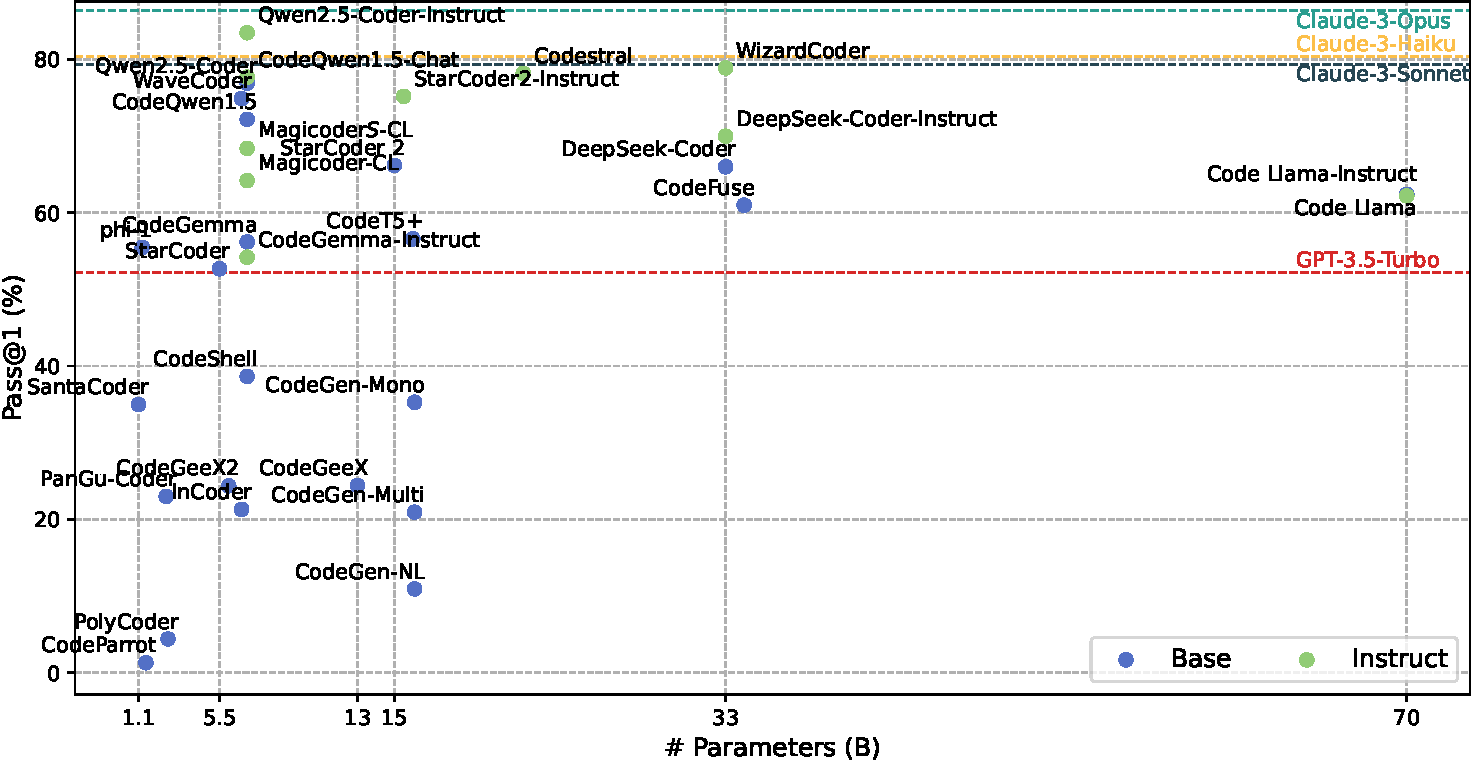
\includegraphics[width=\linewidth]{images/mbpp_scatter.pdf}
\caption{\done{The performance comparison of LLMs for code generation on the MBPP \cite{austin2021program} benchmark, measured by \texttt{Pass@1}. For models with various sizes, we report only the largest size version of each model with a magnitude of \texttt{B} parameters.} 
}
\label{fig:mbpp_performance}
\end{figure*}